\section{实验步骤}

本章节将介绍本实验的步骤,包括数据预处理和数据增强函数、SimpleNet模型、模型预测和损失计算函数、SimpleNet with Dropout模型等。

\subsection{数据预处理和数据增强函数}

数据预处理和数据增强是神经网络训练的重要步骤,它可以提高模型的泛化能力,减少过拟合。在本实验中,使用了数据增强函数,对数据进行了预处理和增强。数据增强函数的代码如下:

\begin{lstlisting}[style=Python]
def get_fundamental_transforms(inp_size, pixel_mean, pixel_std):
    return transforms.Compose([
        transforms.Resize(inp_size),
        transforms.ToTensor(),
        transforms.Normalize(mean=pixel_mean, std=pixel_std),
    ])

def get_data_augmentation_transforms(inp_size, pixel_mean, pixel_std):
    return transforms.Compose([
        transforms.RandomResizedCrop(inp_size),
        # transforms.Resize(inp_size),
        transforms.RandomHorizontalFlip(),
        # transforms.RandomVerticalFlip(),
        transforms.ColorJitter(brightness=0.1, contrast=0.1, saturation=0.1, hue=0.1),
        transforms.ToTensor(),
        transforms.Normalize(mean=pixel_mean, std=pixel_std),
    ])
\end{lstlisting}

上述代码中,\texttt{get\_fundamental\_transforms}函数用于获取基本的数据预处理函数,包括将图像缩放到指定大小、转换为张量、归一化等操作;\texttt{get\_data\_augmentation\_transforms}函数用于获取数据增强函数,其中可选的操作有随机裁剪、随机水平翻转、随机垂直翻转、颜色抖动等。这些操作可以增加数据的多样性,提高模型的泛化能力。Torchvision库提供了丰富的数据增强函数,可以根据实际需求选择合适的操作,而且可以轻松实现数据增强函数的聚合。

\subsection{SimpleNet}

SimpleNet是一个简单的卷积神经网络,由2个卷积层、2个池化层和全连接层组成。SimpleNet的代码如下:

\begin{lstlisting}[style=Python]
class SimpleNet(nn.Module):
    def __init__(self):
        super().__init__()
        self.cnn_layers = nn.Sequential(
            nn.Conv2d(1, 10, kernel_size=(5, 5), stride=(1, 1)),
            nn.MaxPool2d(kernel_size=(3, 3), stride=(3, 3)),
            nn.ReLU(),
            nn.Conv2d(10, 20, kernel_size=(5, 5), stride=(1, 1)),
            nn.MaxPool2d(kernel_size=(3, 3), stride=(3, 3)),
            nn.ReLU())
        self.fc_layers = nn.Sequential(
            nn.Linear(500, 100),
            nn.Linear(100, 15))

    def forward(self, x: torch.tensor) -> torch.tensor:
        x = self.cnn_layers(x)
        x = x.view(x.size(0), -1)
        return self.fc_layers(x)
\end{lstlisting}

上述代码中,\texttt{SimpleNet}包含了\texttt{cnn\_layers}和\texttt{fc\_layers}两个模块。其中,\texttt{cnn\_layers}是卷积神经网络的卷积层和池化层,\texttt{fc\_layers}是全连接层。在\texttt{forward}函数中,首先对输入数据进行卷积和池化操作,然后将输出数据展平,最后通过全连接层得到输出结果。

由于Pytorch提供了丰富的卷积、池化和全连接层的实现,因此可以轻松构建卷积神经网络模型。例如,网络只需要继承\texttt{nn.Module}类,通过\texttt{nn.Conv2d}、\texttt{nn.MaxPool2d}、\texttt{nn.Linear}等类实现卷积、池化和全连接层,然后在\texttt{forward}函数中定义网络的前向传播过程即可。此外,Pytorch提供了\texttt{nn.Sequential}类,可以方便地构建模块的顺序结构,简化了网络的搭建过程。SimpleNet的结构如图\ref{fig:simplenet}所示。

\begin{figure}[H]
    \centering
    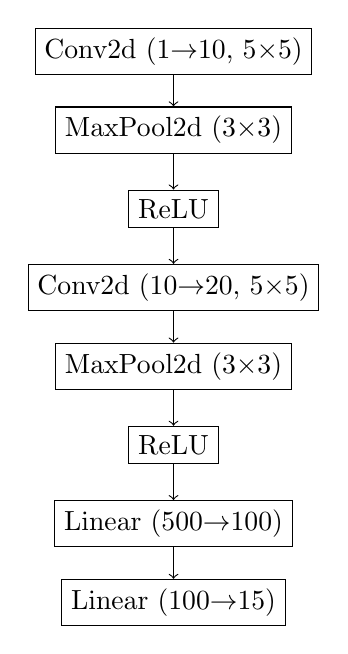
\begin{tikzpicture}
        \node[draw, rectangle] (conv1) {Conv2d (1$\to$10, 5$\times$5)};
        \node[draw, rectangle, below of=conv1] (pool1) {MaxPool2d (3$\times$3)};
        \node[draw, rectangle, below of=pool1] (relu1) {ReLU};
        \node[draw, rectangle, below of=relu1] (conv2) {Conv2d (10$\to$20, 5$\times$5)};
        \node[draw, rectangle, below of=conv2] (pool2) {MaxPool2d (3$\times$3)};
        \node[draw, rectangle, below of=pool2] (relu2) {ReLU};
        \node[draw, rectangle, below of=relu2] (linear1) {Linear (500$\to$100)};
        \node[draw, rectangle, below of=linear1] (linear2) {Linear (100$\to$15)};
        
        \draw[->] (conv1) -- (pool1);
        \draw[->] (pool1) -- (relu1);
        \draw[->] (relu1) -- (conv2);
        \draw[->] (conv2) -- (pool2);
        \draw[->] (pool2) -- (relu2);
        \draw[->] (relu2) -- (linear1);
        \draw[->] (linear1) -- (linear2);
    \end{tikzpicture}
    \caption{SimpleNet网络结构}
    \label{fig:simplenet}
\end{figure}


\newpage
\subsection{模型预测和损失计算函数}

\begin{lstlisting}[style=Python]
def predict_labels(model, x):
    logits = model(x)
    _, predicted_labels = torch.max(logits, 1)
    return predicted_labels


def compute_loss(model, model_output, target_labels, is_normalize):
    # loss = torch.nn.functional.cross_entropy(model_output, target_labels, reduction='sum')
    targets = torch.nn.functional.one_hot(target_labels, num_classes=model_output.size(1))
    loss = - torch.sum(targets * torch.log_softmax(model_output, dim=1), dim=1).sum()
    if is_normalize:
        loss /= model_output.size(0)
    return loss
\end{lstlisting}

上述代码中,\texttt{predict\_labels}函数用于预测模型的输出标签,\newline\texttt{compute\_loss}函数用于计算模型的损失。在\texttt{predict\_labels}函数中,首先通过模型计算输出结果,然后取输出结果中概率最大的标签作为预测标签。在\texttt{compute\_loss}函数中,选择了一种手动的方式来计算损失,而不是通过自带的\texttt{cross\_entropy}函数,从而更便于理解计算过程。交叉熵损失是一种常用的损失函数,用于衡量模型输出与真实标签之间的差异,可以表示为公式\ref{eq:cross_entropy}:

\begin{equation}
    L = -\sum_{i=1}^{N} y_i \log(p_i)
    \label{eq:cross_entropy}
\end{equation}

其中,$y_i$是真实标签的one-hot编码,$p_i$是模型输出的概率。在计算之前,需要将预测分布转换为对数概率,然后与真实标签的独热编码相乘,最后求和得到损失。此外,还可以选择是否对损失进行归一化,以便更好地比较不同批次的损失值。

\subsection{SimpleNet with Dropout}

Dropout是一种常用的正则化技术,用于减少神经网络的过拟合。在本实验中,对SimpleNet模型添加了Dropout层,代码如下:

\begin{lstlisting}[style=Python]
class SimpleNetDropout(nn.Module):
    def __init__(self):
        super().__init__()
        self.cnn_layers = nn.Sequential(
            nn.Conv2d(1, 10, kernel_size=(5, 5), stride=(1, 1), padding=(0, 0)),
            nn.MaxPool2d(kernel_size=(3, 3), stride=(3, 3), padding=0),
            nn.ReLU(),
            nn.Conv2d(10, 20, kernel_size=(5, 5), stride=(1, 1), padding=(0, 0)),
            nn.MaxPool2d(kernel_size=(3, 3), stride=(3, 3), padding=0),
            nn.ReLU())
        self.fc_layers = nn.Sequential(
            nn.Linear(500, 100),
            nn.Dropout(p=0.5),
            nn.Linear(100, 15))

    def forward(self, x: torch.tensor) -> torch.tensor:
        x = self.cnn_layers(x)
        x = x.view(x.size(0), -1)
        return self.fc_layers(x)
\end{lstlisting}

上述代码中,\texttt{SimpleNetDropout}是一个带有Dropout层的SimpleNet模型。在\texttt{fc\_layers}中,添加了一个Dropout层,用于随机丢弃一部分神经元,从而减少模型的过拟合。Dropout层可以在训练过程中随机丢弃神经元,但在测试过程中保留所有神经元,从而提高模型的泛化能力。Dropout层的参数$p$表示丢弃的概率,通常设置为0.5。SimpleNet with Dropout的结构如图\ref{fig:simplenet_dropout}所示。

\begin{figure}[H]
    \centering
    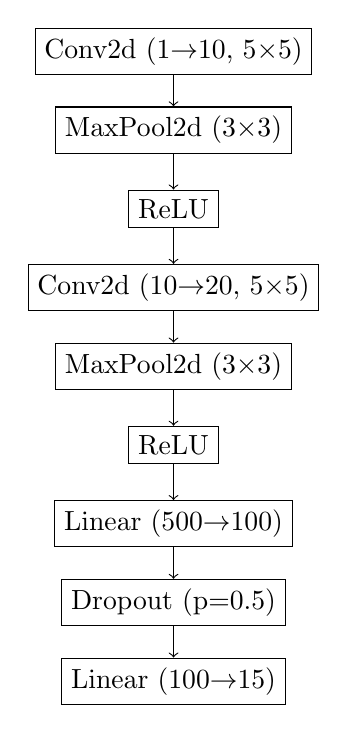
\begin{tikzpicture}
        \node[draw, rectangle] (conv1) {Conv2d (1$\to$10, 5$\times$5)};
        \node[draw, rectangle, below of=conv1] (pool1) {MaxPool2d (3$\times$3)};
        \node[draw, rectangle, below of=pool1] (relu1) {ReLU};
        \node[draw, rectangle, below of=relu1] (conv2) {Conv2d (10$\to$20, 5$\times$5)};
        \node[draw, rectangle, below of=conv2] (pool2) {MaxPool2d (3$\times$3)};
        \node[draw, rectangle, below of=pool2] (relu2) {ReLU};
        \node[draw, rectangle, below of=relu2] (linear1) {Linear (500$\to$100)};
        \node[draw, rectangle, below of=linear1] (dropout) {Dropout (p=0.5)};
        \node[draw, rectangle, below of=dropout] (linear2) {Linear (100$\to$15)};
        
        \draw[->] (conv1) -- (pool1);
        \draw[->] (pool1) -- (relu1);
        \draw[->] (relu1) -- (conv2);
        \draw[->] (conv2) -- (pool2);
        \draw[->] (pool2) -- (relu2);
        \draw[->] (relu2) -- (linear1);
        \draw[->] (linear1) -- (dropout);
        \draw[->] (dropout) -- (linear2);
    \end{tikzpicture}
    \caption{SimpleNet with Dropout网络结构}
    \label{fig:simplenet_dropout}
\end{figure}

\subsection{My Transformer}

Transformer是一种强大的神经网络模型,用于处理序列数据。在本实验中,实现了一个简单的Transformer模型,代码如下:

\begin{lstlisting}[style=Python]
import math
import torch
from functools import partial
from torch import nn
from torch.nn.init import trunc_normal_, _calculate_fan_in_and_fan_out


class MLP(nn.Module):
    def __init__(self,
                 in_features,
                 hid_features,
                 out_features,
                 dropout=0.):
        super(MLP, self).__init__()

        out_features = out_features or in_features
        hid_features = hid_features or in_features

        self.fc1 = nn.Linear(in_features, hid_features)
        self.act = nn.GELU()
        self.fc2 = nn.Linear(hid_features, out_features)
        self.dropout = nn.Dropout(dropout)

    def forward(self, x):
        x = self.fc1(x)
        x = self.act(x)
        x = self.dropout(x)
        x = self.fc2(x)
        x = self.dropout(x)
        return x


class Attention(nn.Module):
    def __init__(self,
                 dim,
                 n_heads=8,
                 qkv_bias=False,
                 attn_dropout=0.,
                 proj_dropout=0.):
        super(Attention, self).__init__()

        self.n_heads = n_heads
        head_dim = dim // n_heads
        self.scale = head_dim ** -.5

        self.qkv = nn.Linear(dim, dim*3, bias=qkv_bias)
        self.attn_dropout = nn.Dropout(attn_dropout)

        self.proj = nn.Linear(dim, dim)
        self.proj_dropout = nn.Dropout(proj_dropout)

    def forward(self, x):
        b, n, c = x.shape
        qkv = self.qkv(x).reshape(b, n, 3, self.n_heads, c//self.n_heads).permute(2, 0, 3, 1, 4)
        q,k,v = qkv[0], qkv[1], qkv[2]

        attn = (q @ k.transpose(-2,-1)) * self.scale
        attn = attn.softmax(dim=-1)
        attn = self.attn_dropout(attn)

        x = (attn @ v).transpose(1,2).reshape(b,n,c)
        x = self.proj(x)
        x = self.proj_dropout(x)
        return x


class EncoderBlock(nn.Module):
    def __init__(self,
                 dim,
                 n_heads,
                 mlp_ratio,
                 qkv_bias=False,
                 dropout=0.,
                 attn_dropout=0.,
                 proj_dropout=0.,
                 norm_layer=nn.LayerNorm):
        super(EncoderBlock, self).__init__()

        self.norm1 = norm_layer(dim)
        self.attn = Attention(dim, n_heads, qkv_bias,
                              attn_dropout, proj_dropout)
        self.dropout = nn.Dropout(dropout)

        self.norm2 = norm_layer(dim)
        mlp_hid_dim = int(dim * mlp_ratio)
        self.mlp = MLP(dim, mlp_hid_dim, dim, dropout)

    def forward(self, x):
        x = x + self.dropout(self.attn(self.norm1(x)))
        x = x + self.dropout(self.mlp(self.norm2(x)))
        return x


class PatchEmbed(nn.Module):

    def __init__(self, img_size=224,
                 patch_size=16,
                 in_c=3,
                 embed_dim=768,
                 norm_layer=None):
        super(PatchEmbed, self).__init__()

        img_size = (img_size, img_size)
        patch_size = (patch_size, patch_size)
        self.img_size = img_size
        self.patch_size = patch_size
        self.grid_size = (img_size[0] // patch_size[0],
                          img_size[1] // patch_size[1])
        self.n_patches = self.grid_size[0] * self.grid_size[1]

        self.proj = nn.Conv2d(in_c, embed_dim,
                              kernel_size=patch_size,
                              stride=patch_size)
        self.norm = norm_layer(embed_dim) if norm_layer else None

    def forward(self, x):
        # (b,c,h,w) -> (b,c,hw) -> (b,hw,c)
        x = self.proj(x).flatten(2).transpose(1, 2)
        if self.norm is not None:
            x = self.norm(x)
        return x


def variance_scaling_(tensor, scale=1.0, mode='fan_in', distribution='normal'):
    fan_in, fan_out = _calculate_fan_in_and_fan_out(tensor)
    if mode == 'fan_in':
        denom = fan_in
    elif mode == 'fan_out':
        denom = fan_out
    elif mode == 'fan_avg':
        denom = (fan_in + fan_out) / 2

    variance = scale / denom

    if distribution == "truncated_normal":
        # constant is stddev of standard normal truncated to (-2, 2)
        trunc_normal_(tensor, std=math.sqrt(variance) / .87962566103423978)
    elif distribution == "normal":
        tensor.normal_(std=math.sqrt(variance))
    elif distribution == "uniform":
        bound = math.sqrt(3 * variance)
        tensor.uniform_(-bound, bound)
    else:
        raise ValueError(f"invalid distribution {distribution}")

def lecun_normal_(tensor):
    variance_scaling_(tensor, mode='fan_in', distribution='truncated_normal')

def init_vit_weights(module, name='', head_bias=0.):
    if isinstance(module, nn.Linear):
        if name.startswith('head'):
            nn.init.zeros_(module.weight)
            nn.init.constant_(module.bias, head_bias)
        elif name.startswith('pre_logits'):
            lecun_normal_(module.weight)
            nn.init.zeros_(module.bias)
        else:
            trunc_normal_(module.weight, std=.02)
            if module.bias is not None:
                nn.init.zeros_(module.bias)
    elif isinstance(module, (nn.LayerNorm, nn.GroupNorm, nn.BatchNorm2d)):
        nn.init.zeros_(module.bias)
        nn.init.ones_(module.weight)


class MyVisionTransformer(nn.Module):
    def __init__(self,
                 img_size=224,
                 patch_size=16,
                 in_c=3,
                 n_classes=1000,
                 embed_dim=768,
                 depth=12,
                 n_heads=12,
                 mlp_ratio=4.,
                 qkv_bias=True,
                 representation_size=None,
                 proj_dropout=0.,
                 attn_dropout=0.,
                 dropout=0.,
                 norm_layer=None):
        super().__init__()

        self.n_classes = n_classes
        self.n_features = self.embed_dim = embed_dim
        self.n_tokens = 1

        norm_layer = norm_layer or partial(nn.LayerNorm, eps=1e-6)
        self.patch_embed = PatchEmbed(img_size, patch_size, in_c, embed_dim)
        n_patches = self.patch_embed.n_patches

        self.cls_token = nn.Parameter(torch.zeros(1, 1, embed_dim))
        self.pos_embed = nn.Parameter(torch.zeros(
            1, n_patches+self.n_tokens, embed_dim))
        self.pos_dropout = nn.Dropout(dropout)

        self.blocks = nn.Sequential(*[
            EncoderBlock(embed_dim, n_heads, mlp_ratio, qkv_bias,
                         dropout, attn_dropout, proj_dropout, norm_layer)
            for _ in range(depth)
        ])

        self.norm = norm_layer(embed_dim)
        self.head = nn.Linear(self.n_features, n_classes)

        nn.init.trunc_normal_(self.pos_embed, std=.02)
        nn.init.trunc_normal_(self.cls_token, std=.02)
        self.apply(init_vit_weights)

    def forward(self, x):
        x = self.patch_embed(x)
        cls_token = self.cls_token.expand(x.shape[0], -1, -1)
        x = torch.cat((cls_token, x), dim=1)

        x = self.pos_dropout(x + self.pos_embed)
        x = self.blocks(x)
        x = self.norm(x)
        x = self.head(x[:, 0])
        return x
\end{lstlisting}

上述代码实现了若干模块,包括MLP、Attention、EncoderBlock、PatchEmbed:

\begin{itemize}
    \item MLP:多层感知机模块,包含两个全连接层和激活函数;
    \item Attention:自注意力模块,用于计算序列数据的注意力权重;
    \item EncoderBlock:编码器模块,包含注意力和MLP两个子模块;
    \item PatchEmbed:图像块嵌入模块,用于将图像分块并嵌入到向量空间中。
\end{itemize}

通过连接上述模块,可以构建一个简单的Transformer模型。在MyVisionTransformer类中,首先通过PatchEmbed模块将图像块嵌入到向量空间中,然后通过多个EncoderBlock模块进行特征提取,最后通过全连接层得到输出结果。Transformer模型的结构如图\ref{fig:transformer}所示。

\begin{figure}[H]
    \centering
    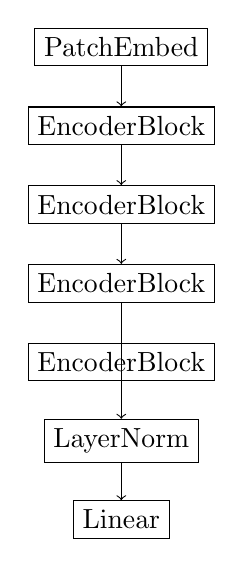
\begin{tikzpicture}
        \node[draw, rectangle] (patch) {PatchEmbed};
        \node[draw, rectangle, below of=patch] (block1) {EncoderBlock};
        \node[draw, rectangle, below of=block1] (block2) {EncoderBlock};
        \node[draw, rectangle, below of=block2] (block3) {EncoderBlock};
        \node[draw, rectangle, below of=block3] (block4) {EncoderBlock};
        \node[draw, rectangle, below of=block4] (norm) {LayerNorm};
        \node[draw, rectangle, below of=norm] (head) {Linear};
        
        \draw[->] (patch) -- (block1);
        \draw[->] (block1) -- (block2);
        \draw[->] (block2) -- (block3);
        \draw[->] (block3) -- (norm);
        \draw[->] (norm) -- (head);
    \end{tikzpicture}
    \caption{Transformer网络结构}
    \label{fig:transformer}
\end{figure}

\subsection{运行脚本}

通过运行如下命令启动jupyter notebook,然后在浏览器中打开链接:

\begin{lstlisting}[style=Bash]
jupyter notebook
\end{lstlisting}

之后打开\texttt{proj4.ipynb}文件,点击如图\ref{fig:jupyter}按钮运行脚本,即可开始实验。

% pics/jupyter.png
\begin{figure}[H]
    \centering
    
\includegraphics[width=0.8\textwidth]{pics/jupyter.png}
    \caption{Jupyter Notebook界面}
    \label{fig:jupyter}
\end{figure}

运行结果如图\ref{fig:unit_test}所示,可以看到所有单元测试均通过,说明实验代码正确。

% 在pics目录中,unit1/2/3/4/5/6.png,6张子图
% 每行2张子图,采用subfloat排列
\begin{figure}[H]
    \centering
    \subfloat[]{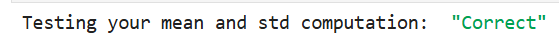
\includegraphics[width=0.4\textwidth]{pics/unit1.png}}
    \subfloat[]{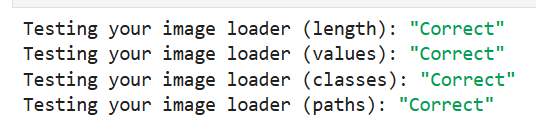
\includegraphics[width=0.4\textwidth]{pics/unit2.png}} \\
    \subfloat[]{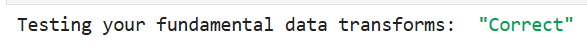
\includegraphics[width=0.4\textwidth]{pics/unit3.png}}
    \subfloat[]{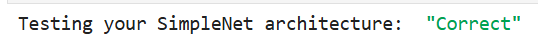
\includegraphics[width=0.4\textwidth]{pics/unit4.png}} \\
    \subfloat[]{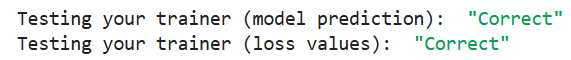
\includegraphics[width=0.4\textwidth]{pics/unit5.png}}
    \subfloat[]{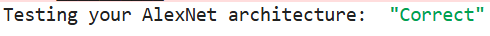
\includegraphics[width=0.4\textwidth]{pics/unit6.png}}
    \caption{单元测试结果}
    \label{fig:unit_test}
\end{figure}